Las tiendas son estructuras que permiten a los jugadores comprar ítems y cosméticos utilizando monedas virtuales 
del juego. Se asignan a estructuras estáticas, por lo que los creadores pueden ubicarlas en cualquier estructura 
dentro de sus mundos, y cada una puede configurarse con un inventario personalizado de ítems y cosméticos 
disponibles para la venta.

\subsubsection{Tiendas}

\begin{figure}[H]
    \centering
    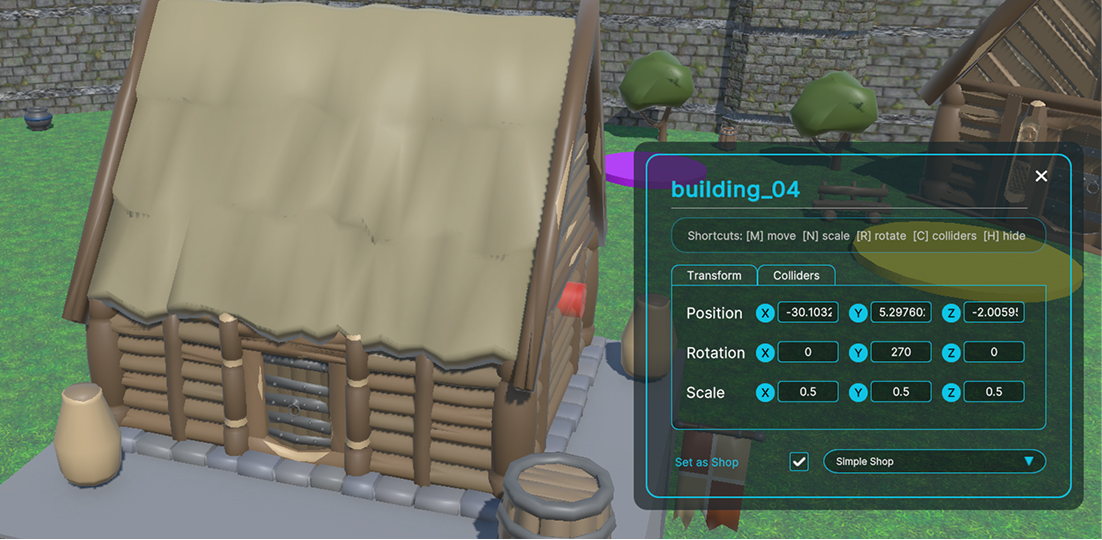
\includegraphics[width=0.8\textwidth]{img/08-implemented-solution/product/shop-structure.jpg}
    \caption{Captura de una estructura siendo asignada como tienda en el creador de mundos}
    \label{fig:shop-structure}
\end{figure}

Los ítems, como armas (\textit{weapons}) o consumibles (\textit{consumables}), se adquieren con oro, una moneda 
virtual específica de cada mundo que no posee valor real, sino que funciona únicamente como moneda dentro del juego. 
Los cosméticos, en cambio, se adquieren con gemas, una moneda virtual que sí tiene valor monetario y que los 
jugadores obtienen mediante la compra de \textit{packs} de gemas en el juego.

\begin{figure}[H]
    \centering
    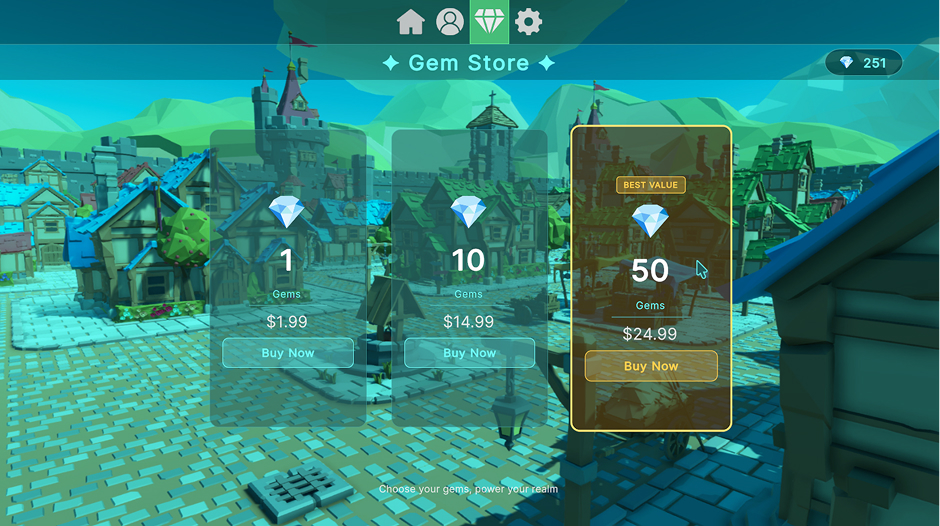
\includegraphics[width=0.85\textwidth]{img/08-implemented-solution/product/gem-store.jpg}
    \caption{Captura de la tienda de gemas en el juego, donde los jugadores pueden comprar packs de gemas con dinero real}
    \label{fig:shop-cosmetics}
\end{figure}

\begin{figure}[H]
    \centering
    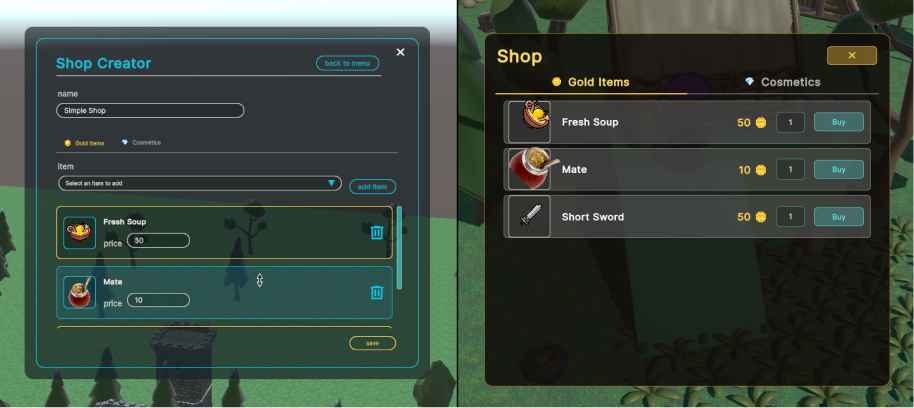
\includegraphics[width=0.85\textwidth]{img/08-implemented-solution/product/shop-items.jpg}
    \caption{Captura del editor de tiendas mostrando ítems disponibles para la venta y como se ve en el juego}
    \label{fig:shop-items}
\end{figure}

\begin{figure}[H]
    \centering
    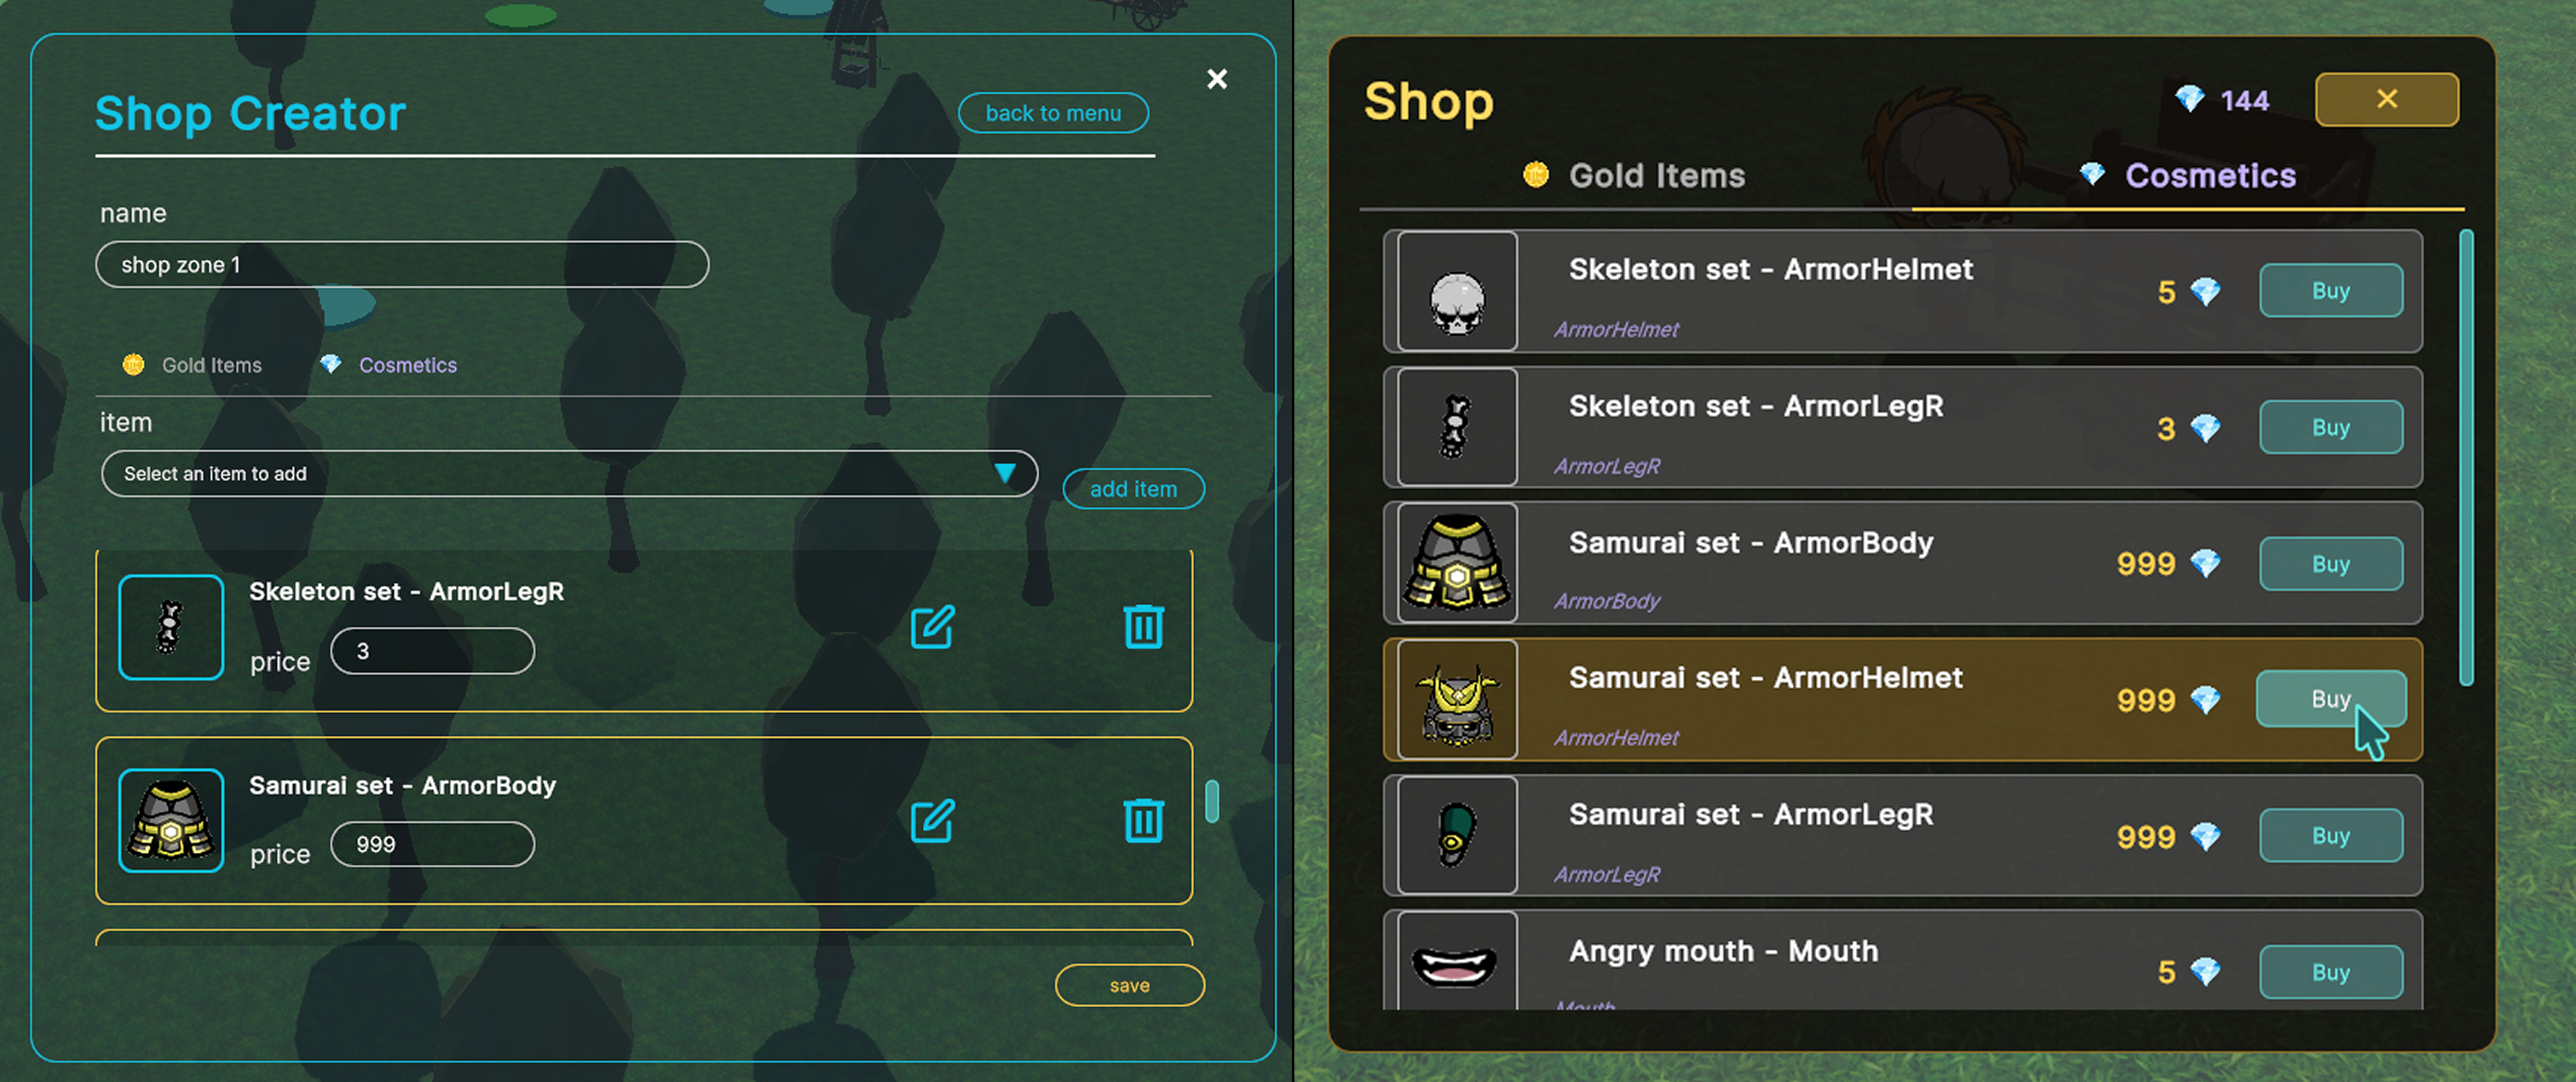
\includegraphics[width=0.85\textwidth]{img/08-implemented-solution/product/shop-cosmetics.jpg}
    \caption{Captura del editor de tiendas mostrando cosméticos disponibles para la venta y como se ve en el juego}
    \label{fig:shop-cosmetics}
\end{figure}

De esta manera, los cosméticos constituyen un elemento clave para la monetización del mundo, ya que permiten a los 
creadores venderlos a cambio de gemas y, posteriormente, convertir esas gemas en dinero real.

\subsubsection{Monetización para creadores}

El creador de mundos cuenta con paneles de gestión económica destinados a los creadores de mundos, que centralizan
el seguimiento de sus mundos publicados. Desde esta sección, el creador puede visualizar el
estado de cada mundo publicado, ver la fecha de renovación de su período de suscripción y
administrar sus publicaciones.
\vspace{0.25cm}

\begin{figure}[H]
\centering
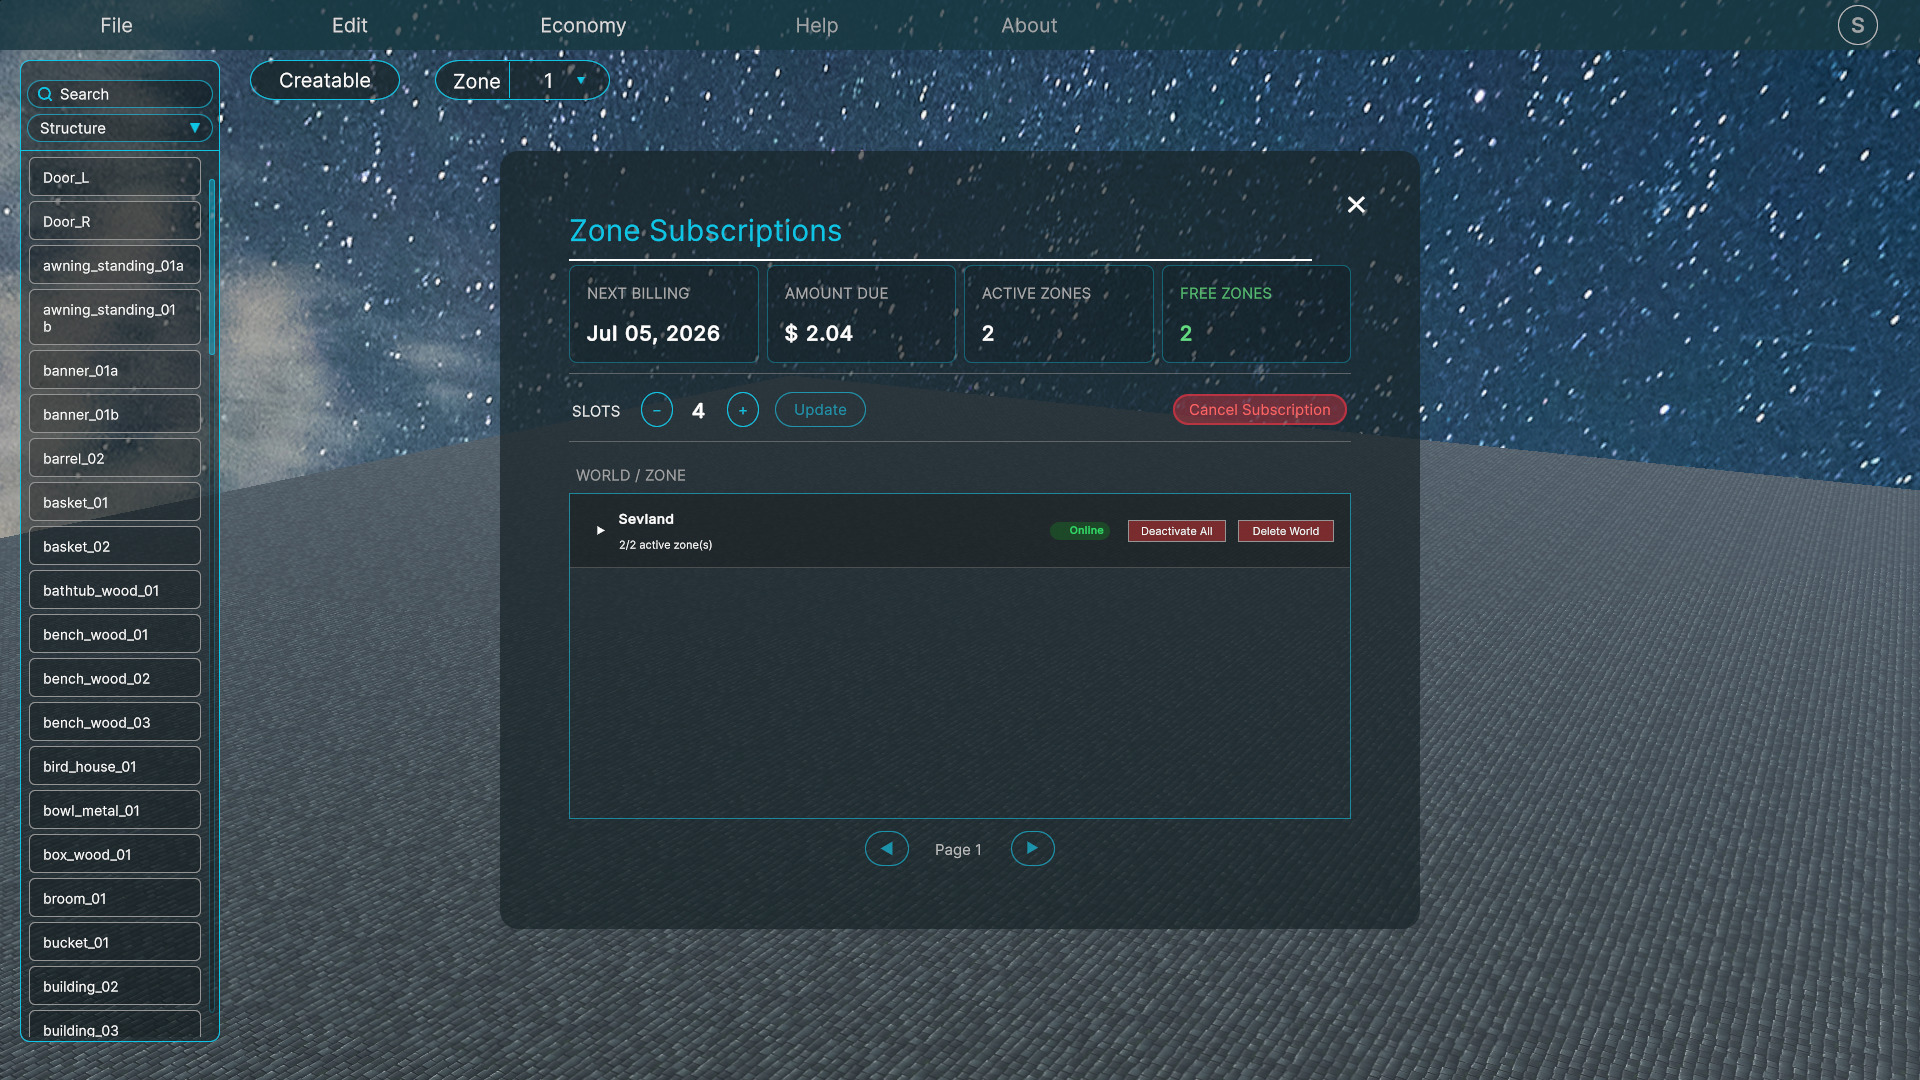
\includegraphics[width=\textwidth]{img/08-implemented-solution/world-editor/subscriptions.jpg}
\caption{Panel de suscripciones.}
\label{fig:subscriptions}
\end{figure}

Adicionalmente, existe un panel de ingresos que permite a los creadores recaudar las
ganancias generadas en sus mundos.